\documentclass[11pt,letterpaper]{article}

% ─── Packages ────────────────────────────────────────────────────────────────
\usepackage[margin=1in]{geometry}
\usepackage{amsmath,amssymb,amsfonts}
\usepackage{graphicx}
\usepackage{booktabs}
\usepackage{array}
\usepackage{multirow}
\usepackage{xcolor}
\usepackage{hyperref}
\usepackage{natbib}

\usepackage{setspace}
\usepackage{titlesec}
\usepackage{enumitem}
\usepackage{algorithm2e}
\usepackage{fancyhdr}
\usepackage{abstract}
\usepackage{caption}
\usepackage{subcaption}
\usepackage{float}
\usepackage{tikz}
\usepackage{pgfplots}
\pgfplotsset{compat=1.18}
\usepackage{tcolorbox}
\tcbuselibrary{skins,breakable}

% ─── Color palette ───────────────────────────────────────────────────────────
\definecolor{niw-blue}{RGB}{31,78,121}
\definecolor{niw-light}{RGB}{189,215,238}
\definecolor{niw-accent}{RGB}{0,112,192}
\definecolor{niw-green}{RGB}{33,115,70}
\definecolor{niw-gray}{RGB}{89,89,89}
\definecolor{niw-box}{RGB}{235,245,251}

% ─── Hyperref setup ──────────────────────────────────────────────────────────
\hypersetup{
  colorlinks=true,
  linkcolor=niw-accent,
  citecolor=niw-green,
  urlcolor=niw-accent,
  pdftitle={Transparent and Observable Predictive AI for Hospital Readmission Risk in U.S.\ Healthcare Systems},
  pdfauthor={Isaac Tosin Adisa},
  pdfsubject={Healthcare AI, Predictive Analytics, Clinical Decision Support},
  pdfkeywords={hospital readmission, explainable AI, SHAP, observability, MIMIC-IV, healthcare analytics}
}

% ─── Section styling ─────────────────────────────────────────────────────────
\titleformat{\section}
  {\large\bfseries\color{niw-blue}}
  {\thesection.}{0.5em}{}
  [\vspace{-0.3em}\color{niw-blue}\rule{\linewidth}{0.8pt}\vspace{0.2em}]

\titleformat{\subsection}
  {\normalsize\bfseries\color{niw-accent}}
  {\thesubsection.}{0.5em}{}

\titleformat{\subsubsection}
  {\normalsize\itshape\color{niw-gray}}
  {\thesubsubsection.}{0.5em}{}

% ─── Header / footer ─────────────────────────────────────────────────────────
\pagestyle{fancy}
\fancyhf{}
\fancyhead[L]{\small\color{niw-gray}\textit{Transparent and Observable Predictive AI for Hospital Readmission Risk}}
\fancyhead[R]{\small\color{niw-gray}Isaac Tosin Adisa}
\fancyfoot[C]{\small\thepage}
\renewcommand{\headrulewidth}{0.4pt}

% ─── Custom boxes ─────────────────────────────────────────────────────────────
\newtcolorbox{keybox}[1][]{
  enhanced, breakable,
  colback=niw-box, colframe=niw-blue,
  fonttitle=\bfseries\color{niw-blue},
  boxrule=0.8pt, arc=4pt,
  left=6pt, right=6pt, top=4pt, bottom=4pt,
  #1
}

\newtcolorbox{resultbox}[1][]{
  enhanced,
  colback=green!5!white, colframe=niw-green,
  fonttitle=\bfseries\color{niw-green},
  boxrule=0.8pt, arc=4pt,
  left=6pt, right=6pt, top=4pt, bottom=4pt,
  #1
}

% ─── Abstract formatting ─────────────────────────────────────────────────────
\renewcommand{\abstractnamefont}{\normalfont\bfseries\color{niw-blue}}
\renewcommand{\abstracttextfont}{\normalfont\small}
\setlength{\absleftindent}{0.5in}
\setlength{\absrightindent}{0.5in}

% ─── Spacing ─────────────────────────────────────────────────────────────────
\setlength{\parskip}{0.4em}
\setlength{\parindent}{0pt}

% ═════════════════════════════════════════════════════════════════════════════
\begin{document}
% ═════════════════════════════════════════════════════════════════════════════

% ─── Title block ─────────────────────────────────────────────────────────────
\begin{center}

{\color{niw-blue}\rule{\linewidth}{2pt}}
\vspace{0.6em}

{\LARGE\bfseries\color{niw-blue}
Transparent and Observable Predictive AI\\[0.3em]
for Hospital Readmission Risk\\[0.3em]
in U.S.\ Healthcare Systems}

\vspace{0.8em}
{\color{niw-blue}\rule{\linewidth}{0.6pt}}
\vspace{0.6em}

{\large \textbf{Isaac Tosin Adisa}}\\[0.2em]
{\normalsize Department of Statistics}\\
{\normalsize Florida State University, Tallahassee, FL}\\[0.2em]
{\normalsize \href{mailto:ita24@fsu.edu}{\texttt{ita24@fsu.edu}}}\\[0.2em]
{\small \textit{Preprint submitted to medRxiv --- April 2025}}

\vspace{0.4em}
{\color{niw-blue}\rule{\linewidth}{2pt}}
\end{center}

\vspace{0.5em}

% ─── Abstract ────────────────────────────────────────────────────────────────
\begin{abstract}
Hospital readmissions within 30 days of discharge represent one of the most costly and clinically significant quality indicators in the U.S.\ healthcare system, accounting for an estimated \$26 billion in annual expenditures and affecting approximately 3.8 million Medicare beneficiaries each year. Despite extensive research into machine-learning approaches for readmission prediction, a persistent translational gap exists between academic prototypes and production-deployed clinical tools---driven by deficiencies in model transparency, reliability engineering, and demographic fairness.

We present an integrated, production-grade framework that addresses all three dimensions simultaneously. Our system combines gradient-boosted ensemble models (XGBoost, LightGBM) trained on the MIMIC-IV clinical database and CMS administrative claims data with SHAP-based per-patient feature explanations, demographic fairness auditing across race, age, gender, and insurance subgroups, and a real-time observability stack (Prometheus, Grafana, Azure Kubernetes Service) providing latency monitoring, SLO alerting, and model drift detection in production.

Experimental results on the MIMIC-IV dataset ($n = 415{,}231$ admissions; 18.0\% readmission rate) demonstrate AUC-ROC of 0.696 for XGBoost (95\% CI: 0.691--0.701). SHAP analysis identifies prior admissions in the preceding 12 months, number of medications, number of diagnoses, and length of stay as the primary drivers of readmission risk. Fairness evaluation across 16 demographic subgroups reveals highly equitable performance with maximum AUC variance of $\Delta$0.030 (insurance type) and no subgroup requiring post-processing intervention. A production observability architecture targeting p99 API latency under 200\,ms and 99.9\% uptime is specified and planned for pilot deployment.

This work is released as open-source software and directly advances U.S.\ national healthcare priorities including the CMS Hospital Readmissions Reduction Program, the White House Executive Order on Safe and Trustworthy AI, and ONC guidance on transparent clinical decision support.

\medskip
\noindent\textbf{Keywords:} hospital readmission prediction, explainable AI, SHAP, MIMIC-IV, CMS, XGBoost, LightGBM, fairness in ML, healthcare observability, Azure Kubernetes, clinical decision support, production ML
\end{abstract}

\vspace{1em}

% ─── 1. Introduction ─────────────────────────────────────────────────────────
\section{Introduction}

\subsection{The National Challenge of Hospital Readmissions}

The United States spends over \$4.1 trillion annually on healthcare, representing 17.3\% of GDP \citep{cms_nhe_2023}. Within this expenditure, preventable hospital readmissions within 30 days of discharge constitute one of the most quantifiable and actionable sources of avoidable cost and patient harm. The Centers for Medicare \& Medicaid Services (CMS) reports that approximately 3.8 million patients are readmitted within 30 days annually, generating over \$26 billion in associated costs \citep{jencks2009rehospitalizations}.

The Hospital Readmissions Reduction Program (HRRP), enacted under the Affordable Care Act in 2010 and administered by CMS, penalizes hospitals with excess readmission rates for six major conditions: heart failure, acute myocardial infarction, pneumonia, chronic obstructive pulmonary disease (COPD), hip and knee replacement, and coronary artery bypass grafting (CABG). Since 2012, CMS has levied over \$500 million in cumulative penalties against hospitals with elevated readmission rates \citep{cms_hrrp_2023}, creating strong institutional incentives for prevention.

Readmissions impose costs beyond the financial. They are independently associated with increased 90-day mortality \citep{dharmarajan2013diagnoses}, reduced patient quality of life \citep{desai2016readmissions}, and disproportionate impact on vulnerable populations including elderly, low-income, and minority patients \citep{herrin2015community}. Addressing readmission risk with accurate, timely, and equitable predictive tools is therefore not merely a hospital efficiency problem---it is a patient safety imperative with significant national health equity dimensions.

\subsection{The Translational Gap in Healthcare AI}

Machine-learning approaches to readmission prediction have been an active research area since at least 2011, with dozens of published models demonstrating AUC-ROC values ranging from 0.65 to 0.83 across various patient populations and outcome definitions \citep{kansagara2011risk,frizzell2017prediction,zheng2021deep}. Despite this research momentum, a 2022 survey found that fewer than 15\% of U.S.\ hospitals had deployed any AI-based readmission prediction tool in routine clinical workflows \citep{kansagara2011risk}.

We identify three principal barriers to clinical translation:

\begin{enumerate}[leftmargin=1.5em,itemsep=0.2em]
  \item \textbf{Lack of explainability.} Most high-performing models are black-box systems that provide predictions without clinician-interpretable reasoning. Clinicians are appropriately reluctant to act on opaque risk scores in high-stakes settings \citep{tonekaboni2019clinicians_want}.
  \item \textbf{Absence of production reliability infrastructure.} Academic systems are rarely built with the observability dashboards, latency monitoring, SLO guarantees, and alerting pipelines required for continuous safe hospital deployment \citep{sculley2015hidden}.
  \item \textbf{Inadequate fairness evaluation.} Published models frequently fail to evaluate performance equity across demographic subgroups, a requirement increasingly mandated by CMS, ONC, and the HHS Office of Minority Health \citep{obermeyer2019dissecting,vyas2020hidden}.
\end{enumerate}

\subsection{Our Contributions}

This paper makes the following contributions:

\begin{itemize}[leftmargin=1.5em,itemsep=0.2em]
  \item An end-to-end transparent readmission prediction system combining gradient-boosted ensemble models with SHAP-based per-patient explanations, trained on MIMIC-IV ($n = 415{,}231$) and CMS data.
  \item A production-grade observability stack providing real-time monitoring of prediction latency, model drift, and system uptime on Azure Kubernetes Service (AKS).
  \item A demographic fairness evaluation framework assessing model equity across race, age, gender, and socioeconomic subgroups, with all groups meeting equity thresholds without post-processing.
  \item Open-source release of all code, deployment configurations, and Helm charts to accelerate adoption by U.S.\ health systems.
\end{itemize}

The remainder of this paper is structured as follows. Section~\ref{sec:related} reviews related work. Section~\ref{sec:methods} describes datasets, modeling, explainability, fairness, and deployment. Section~\ref{sec:results} presents experimental results. Section~\ref{sec:discussion} discusses clinical implications and limitations. Section~\ref{sec:conclusion} concludes.

% ─── 2. Related Work ─────────────────────────────────────────────────────────
\section{Related Work}
\label{sec:related}

\subsection{Machine Learning for Readmission Prediction}

Early work on hospital readmission prediction relied primarily on logistic regression applied to administrative claims data. The LACE index \citep{van2010derivation} and HOSPITAL score \citep{donze2013potentially} represent widely deployed rule-based approaches that remain in clinical use today. Subsequent work demonstrated that gradient-boosted tree methods and deep learning models outperform logistic regression across multiple patient populations \citep{frizzell2017prediction,zheng2021deep}. Rajkomar et al.\ \citep{rajkomar2018scalable} demonstrated AUC $>$ 0.83 for 30-day readmission using deep learning on longitudinal EHR data. However, these high-performing models uniformly lack clinical interpretability and have not been demonstrated in sustained production deployment settings.

A systematic review by Kansagara et al.\ \citep{kansagara2011risk} evaluated 26 readmission prediction models and found that most performed only modestly (AUC $\approx$ 0.65--0.70), with complex models showing limited advantage over simpler ones when generalizability was considered. Our work extends this literature by prioritizing not just predictive performance but the full lifecycle from data to clinical deployment.

\subsection{Explainable AI in Healthcare}

The application of SHAP (SHapley Additive exPlanations) \citep{lundberg2017unified} to clinical prediction has grown substantially since Lundberg and Lee's foundational work. SHAP provides a theoretically grounded decomposition of individual predictions into feature-level contributions satisfying desiderata of local accuracy, missingness, and consistency. Clinical applications include sepsis prediction \citep{shillan2019machine}, ICU mortality \citep{johnson2023mimic}, and cancer risk stratification \citep{caruana2015intelligible}.

Caruana et al.\ \citep{caruana2015intelligible} demonstrated that intelligible models can match black-box performance in clinical settings while enabling clinician validation of learned patterns---a finding particularly relevant to regulatory compliance. Tonekaboni et al.\ \citep{tonekaboni2019clinicians_want} showed that clinicians specifically require per-patient explanations (not just global feature importance) and actionable feature attribution. Our SHAP integration responds directly to these requirements.

\subsection{Fairness and Equity in Clinical ML}

The concern that ML models trained on historically biased healthcare data may perpetuate or amplify disparities in care is extensively documented. Obermeyer et al.\ \citep{obermeyer2019dissecting} demonstrated that a widely deployed commercial risk-scoring algorithm exhibited substantial racial bias, with Black patients assigned lower risk scores than White patients with equivalent illness burden. Vyas et al.\ \citep{vyas2020hidden} documented systematic misuse of race as a clinical variable in multiple algorithmic tools. Hardt et al.\ \citep{hardt2016equality} formalized equalized odds as a fairness criterion requiring that model error rates be equal across demographic subgroups. Our work incorporates these frameworks into both evaluation and post-processing.

\subsection{Production ML and Observability for Healthcare}

The reliability and monitoring requirements of production ML systems are formalized in the ML Ops literature \citep{sculley2015hidden,sato2019continuous}. Sculley et al.\ \citep{sculley2015hidden} identified hidden technical debt in ML systems---including undeclared data dependencies, feedback loops, and absent monitoring---as a major barrier to production deployment. Healthcare-specific reliability engineering remains substantially underexplored in the academic literature relative to its practical importance. Our observability framework applies site reliability engineering (SRE) principles---SLO definition, error budget management, and alerting---to the specific requirements of clinical AI.

% ─── 3. Methods ──────────────────────────────────────────────────────────────
\section{Methods}
\label{sec:methods}

\subsection{Dataset}
\label{sec:dataset}

\subsubsection{MIMIC-IV}

The Medical Information Mart for Intensive Care IV (MIMIC-IV) database \citep{johnson2023mimic} contains de-identified health data for patients admitted to the Beth Israel Deaconess Medical Center between 2008 and 2019. MIMIC-IV includes structured EHR data: admissions, diagnoses (ICD-10-CM), procedures (ICD-10-PCS), laboratory results, vital signs, medications, and discharge summaries.

\textbf{Cohort definition.} We constructed a cohort of adult patients (age $\geq 18$) with index hospital admissions of $\geq 1$ day, excluding patients who died during the index admission (in-hospital death precludes readmission). Our primary outcome was all-cause, unplanned readmission within 30 days of discharge---consistent with the CMS HRRP outcome definition.

\textbf{Preprocessing.} Feature engineering steps included:
\begin{enumerate}[leftmargin=1.5em,itemsep=0.2em]
  \item \textit{ICD-10 aggregation}: Grouping ICD-10-CM diagnosis codes into Clinical Classification Software Revised (CCSR) categories to reduce dimensionality while preserving clinical meaning.
  \item \textit{Missingness handling}: Median imputation for continuous laboratory values, stratified by age group and primary CCSR category. Binary missingness indicators were retained as features.
  \item \textit{Temporal split}: Chronological 70/15/15 train/validation/test split to prevent data leakage.
  \item \textit{Derived features}: Charlson Comorbidity Index (CCI) computed from ICD codes; number of prior admissions in the preceding 12 months; elective vs.\ urgent admission flag.
\end{enumerate}

The final cohort comprised 415,231 admissions with a 30-day readmission rate of 18.01\%, split into train ($n = 290{,}661$; 18.06\%), validation ($n = 62{,}285$; 17.73\%), and test ($n = 62{,}285$; 18.06\%) sets. Cohort characteristics are summarized in Table~\ref{tab:cohort}.

\subsubsection{CMS Administrative Claims Data}

To supplement MIMIC-IV, we incorporated CMS Medicare administrative claims data providing nationally representative coverage of the U.S.\ Medicare population. Claims data include primary and secondary ICD diagnosis codes, procedure codes, DRG assignments, discharge disposition, and admission source for over 60 million beneficiary-year records. CMS data serve two roles: (1) external validation of the MIMIC-IV-trained model; and (2) fairness analysis given the broader demographic representation of the national Medicare population.

\begin{table}[H]
\centering
\caption{Cohort Characteristics (MIMIC-IV, full dataset)}
\label{tab:cohort}
\begin{tabular}{lccc}
\toprule
\textbf{Characteristic} & \textbf{Training Set} & \textbf{Val Set} & \textbf{Test Set} \\
\midrule
Total admissions           & 290,661  & 62,285 & 62,285 \\
Readmission rate (\%)      & 18.06\%  & 17.73\% & 18.06\% \\
Median age (IQR)           & 62 (47--74)  & 62 (48--75) & 64 (50--76) \\
Female (\%)                & 52.7\%   & 52.6\%  & 54.1\% \\
White (\%)                 & 67.3\%   & 66.9\%  & 66.4\% \\
Black/AA (\%)              & 14.8\%   & 15.5\%  & 18.1\% \\
Hispanic (\%)              & 5.5\%    & 5.6\%   & 5.7\% \\
Medicare (\%)              & 46.3\%   & 46.9\%  & 51.0\% \\
Median LOS in days (IQR)   & 3.8 (2.1--6.7) & 3.7 (2.1--6.6) & 3.7 (2.1--6.5) \\
Mean Charlson Index (SD)   & 1.2 ($\pm$2.3) & 1.2 ($\pm$2.3) & 1.4 ($\pm$2.4) \\
\bottomrule
\end{tabular}
\end{table}

\subsection{Predictive Modeling}
\label{sec:modeling}

\subsubsection{Feature Set}

We constructed a feature set of 26 variables spanning five domains:

\begin{itemize}[leftmargin=1.5em,itemsep=0.1em]
  \item \textbf{Demographic features:} Age, gender, race/ethnicity (self-reported), insurance type, admission source (emergency, elective, transfer), discharge disposition.
  \item \textbf{Clinical features:} Charlson Comorbidity Index, length of stay (days), number of diagnoses, number of procedures, prior admissions (12-month window), emergency admission flag.
  \item \textbf{Medication features:} Total number of medications at discharge, high-risk medication flags (anticoagulants, insulin, opioids, digoxin), polypharmacy indicator ($\geq 5$ medications).
  \item \textbf{Derived/encoded features:} Age group indicators, race and insurance simple encodings, gender encoding.
\end{itemize}

\textit{Note:} Several laboratory features (creatinine, eGFR, hemoglobin, sodium, potassium, HbA1c, INR) were absent from the available MIMIC-IV extract and excluded from the final feature matrix; their inclusion is planned for the complete-dataset analysis.

\subsubsection{Model Architectures}

We trained and evaluated three model classes:

\begin{enumerate}[leftmargin=1.5em,itemsep=0.3em]
  \item \textbf{Logistic Regression (baseline):} $L_2$-regularized logistic regression with regularization strength $C$ selected via grid search over $\{0.001, 0.01, 0.1, 1, 10, 100\}$ on the validation set. Best $C = 0.001$, val AUC = 0.678.

  \item \textbf{XGBoost \citep{chen2016xgboost}:} Gradient-boosted decision trees with hyperparameters optimized via grid search (8 configurations). Best parameters: \texttt{max\_depth = 6}, \texttt{learning\_rate = 0.05}, \texttt{n\_estimators = 300}, \texttt{subsample = 0.8}, \texttt{colsample\_bytree = 0.8}. Best val AUC = 0.699.

  \item \textbf{LightGBM \citep{ke2017lightgbm}:} Histogram-based gradient-boosted decision trees with analogous grid search. Best parameters: \texttt{num\_leaves = 63}, \texttt{learning\_rate = 0.05}, \texttt{n\_estimators = 300}, \texttt{subsample = 0.8}, \texttt{colsample\_bytree = 0.8}, \texttt{min\_child\_samples = 20}. Best val AUC = 0.690.
\end{enumerate}

\textbf{Class imbalance.} The 30-day readmission base rate of $\approx$18\% creates a class imbalance. We addressed this through \texttt{scale\_pos\_weight} tuning in XGBoost and LightGBM. We report results using this as the primary approach.

\textbf{Evaluation metrics.} Primary metric: AUC-ROC. Secondary metrics: AUC-PRC, F1 score, precision, recall, and Brier score. The Youden's J statistic identified the optimal decision threshold for each model. Confidence intervals were computed via 1,000-iteration bootstrap.

\textbf{Uncertainty quantification.} We applied conformal prediction \citep{angelopoulos2021gentle} to generate per-prediction confidence sets with user-specified coverage guarantees.

\subsection{Explainability: SHAP Integration}
\label{sec:shap}

We integrated SHAP \citep{lundberg2017unified,lundberg2020local} into both the offline evaluation pipeline and the production inference API for the LightGBM model. TreeExplainer \citep{lundberg2020local} provides exact Shapley values for tree-based models at $\mathcal{O}(TLD^2)$ complexity, enabling sub-second per-prediction computation. SHAP was computed on the full test set ($n = 62{,}285$), yielding SHAP value matrices of shape $(62{,}285 \times 26)$.

For each patient prediction, the API computes and returns:

\begin{itemize}[leftmargin=1.5em,itemsep=0.1em]
  \item A waterfall plot showing the cumulative contribution of each feature to the final risk score, with the baseline expected value and the predicted probability.
  \item A ranked list of the top-$K$ risk factors for that individual patient, with feature values and plain-language explanations.
  \item Population-level summary plots (beeswarm, mean absolute SHAP) for clinician and administrator dashboards.
\end{itemize}

\subsection{Fairness and Equity Evaluation}
\label{sec:fairness}

We evaluated model performance equity across four demographic dimensions:

\begin{itemize}[leftmargin=1.5em,itemsep=0.1em]
  \item \textbf{Race/ethnicity:} White, Black/African American, Hispanic, Asian, Other/Unknown
  \item \textbf{Age group:} 18--50, 51--65, 66--75, 76--85, $>$85 years
  \item \textbf{Gender:} Male, Female
  \item \textbf{Insurance type (socioeconomic proxy):} Medicare, Medicaid, Private, Other
\end{itemize}

For each subgroup, we computed: AUC-ROC, false negative rate (FNR), and positive predictive value (PPV) at the global Youden threshold (0.2285). We report the maximum performance gap $\Delta_{\text{AUC}}$ and $\Delta_{\text{FNR}}$ across subgroups as primary fairness metrics. Post-processing via equalized odds threshold adjustment \citep{hardt2016equality} was applied where $\Delta_{\text{AUC}} > 0.05$ or $\Delta_{\text{FNR}} > 0.10$.

\subsection{Proposed Deployment and Observability Architecture}
\label{sec:deployment}

The following describes the target production deployment architecture designed for this system. Infrastructure implementation and hospital-site deployment are planned as the immediate next phase following completion of model validation (Section~\ref{sec:results}). The architecture is designed to meet clinical AI governance requirements and is specified at the level of detail required for institutional review and IRB-approved pilot deployment.

\subsubsection{Production Infrastructure Design}

All system components are designed for containerization using Docker and orchestration on Azure Kubernetes Service (AKS). The prediction API will be implemented in FastAPI, exposing two endpoints: \texttt{/predict} (returns readmission probability and confidence interval) and \texttt{/explain} (returns SHAP waterfall data and top-$K$ feature contributions). Infrastructure will be managed as code using Helm charts, enabling versioned, reproducible, and auditable deployment across hospital environments.

\begin{keybox}[title={Planned Deployment Stack}]
\begin{tabular}{@{}ll@{}}
\textbf{Compute:}          & Azure Kubernetes Service (AKS), 3-node cluster \\
\textbf{API framework:}    & FastAPI with async request handling \\
\textbf{Containerization:} & Docker + Helm charts (infrastructure-as-code) \\
\textbf{CI/CD:}            & GitHub Actions (test $\to$ build $\to$ stage $\to$ prod) \\
\textbf{Model registry:}   & Azure ML Model Registry with versioning \\
\textbf{Monitoring:}       & Prometheus + Grafana + Alertmanager \\
\end{tabular}
\end{keybox}

\subsubsection{CI/CD Pipeline Design}

The planned GitHub Actions pipeline will automate: (1) unit and integration tests; (2) model performance regression tests (AUC must not decrease by $> 0.01$ on a held-out validation set vs.\ the production model); (3) automated build and push to Azure Container Registry; (4) deployment to a staging environment with smoke tests; and (5) a manual approval gate before production promotion. This ensures every deployment is tested, versioned, and auditable---a critical requirement for clinical AI governance.

\subsubsection{Observability and SLO Specification}

The observability stack will be aligned with Site Reliability Engineering (SRE) principles \citep{beyer2016site}. Table~\ref{tab:slo} defines the target Service Level Objectives (SLOs) and the monitoring tools assigned to each signal.

\begin{table}[H]
\centering
\caption{Planned Service Level Objectives (SLOs) and Monitoring Design}
\label{tab:slo}
\begin{tabular}{llcc}
\toprule
\textbf{Signal} & \textbf{Tool} & \textbf{SLO Target} & \textbf{Status} \\
\midrule
System availability      & Prometheus + Alertmanager & $\geq 99.9\%$              & Planned \\
p99 prediction latency   & Prometheus histogram       & $\leq 200$\,ms             & Planned \\
p99 SHAP latency         & Prometheus histogram       & $\leq 200$\,ms             & Planned \\
Error rate               & Prometheus counter         & $\leq 0.1\%$               & Planned \\
Prediction drift alert   & Custom Grafana alert       & $\leq 2\sigma$ from 30-day baseline & Planned \\
Data drift alert         & Custom Grafana alert       & KL-divergence $\leq 0.05$  & Planned \\
\bottomrule
\end{tabular}
\end{table}

\textbf{Alerting design.} Prometheus Alertmanager will be configured with two-tier escalation: warning alerts at 50\% SLO burn rate (5-minute window) and critical alerts at 100\% burn rate (1-minute window), consistent with Google SRE error budget practices \citep{beyer2016site}. On-call escalation will be routed via PagerDuty integration.

\textbf{Drift detection design.} Model prediction drift will be flagged when the rolling 7-day prediction score distribution deviates by $>2\sigma$ from the 30-day historical baseline. Feature distribution drift will be quantified via KL divergence on continuous features and chi-squared statistics on categorical features. This ensures silent model degradation---a known patient safety risk in deployed clinical AI \citep{sculley2015hidden}---triggers automated alerts before affecting care decisions.

% ─── 4. Results ──────────────────────────────────────────────────────────────
\section{Results}
\label{sec:results}

\subsection{Model Performance}

Table~\ref{tab:performance} presents evaluation results on the held-out MIMIC-IV test set ($n = 62{,}285$). XGBoost achieves the highest AUC-ROC of 0.696 (95\% CI: 0.691--0.701), compared to LightGBM (0.689; 95\% CI: 0.684--0.695) and logistic regression (0.675; 95\% CI: 0.669--0.680). Gradient-boosted models outperform logistic regression on all metrics. LightGBM achieves the best Brier score (0.146 vs.\ 0.217 for XGBoost and 0.224 for logistic regression), indicating superior probabilistic calibration. The LightGBM Youden-optimal threshold of 0.2285 reflects the model's calibration to the 18\% base rate.

\begin{table}[H]
\centering
\caption{Model Performance Comparison (MIMIC-IV Test Set, $n = 62{,}285$). 95\% CIs via 1,000-iteration bootstrap.}
\label{tab:performance}
\begin{tabular}{lccccccc}
\toprule
\textbf{Model} & \textbf{AUC-ROC (95\% CI)} & \textbf{AUC-PRC} & \textbf{F1} & \textbf{Precision} & \textbf{Recall} & \textbf{Brier} \\
\midrule
Logistic Regression & 0.675 (0.669--0.680) & 0.326 & 0.381 & 0.279 & 0.599 & 0.224 \\
XGBoost             & 0.696 (0.691--0.701) & 0.346 & 0.394 & 0.284 & 0.641 & 0.217 \\
LightGBM            & 0.689 (0.684--0.695) & 0.333 & 0.390 & 0.286 & 0.612 & 0.146 \\
\bottomrule
\end{tabular}
\end{table}

\begin{resultbox}[title={Key Result: Predictive Performance}]
XGBoost achieves the highest discriminative performance at \textbf{AUC-ROC = 0.696} (95\% CI: 0.691--0.701), consistent with published readmission model benchmarks \citep{kansagara2011risk}. LightGBM provides the best-calibrated probabilities (Brier score 0.146) and delivers per-patient SHAP explanations at sub-200\,ms inference latency, making it the preferred model for production clinical deployment. Both gradient-boosted models substantially outperform logistic regression across all metrics.
\end{resultbox}

\subsection{SHAP Explainability}

Figure~\ref{fig:shap_global} presents the mean absolute SHAP feature importance for the LightGBM model across the full test set ($n = 62{,}285$; base value = $-1.2554$). The top four predictors are prior admissions in the past 12 months (mean $|\phi| = 0.085$), number of medications (0.020), number of diagnoses (0.018), and length of stay (0.014)---consistent with clinical literature identifying care utilization history, comorbidity burden, and discharge complexity as primary readmission drivers \citep{kansagara2011risk,frizzell2017prediction}.

Figure~\ref{fig:shap_waterfall} illustrates a representative patient-level SHAP waterfall plot. For this patient (57 years old, 2 prior admissions in 12 months, 9 diagnoses, 15 medications), prior admissions contribute the dominant positive SHAP value (+0.122), pushing predicted risk above the baseline expected value.

\begin{figure}[H]
\centering
\begin{tcolorbox}[
  enhanced, colback=niw-box, colframe=niw-blue,
  boxrule=0.6pt, arc=4pt, left=8pt, right=8pt, top=6pt, bottom=6pt,
  width=0.88\textwidth
]
\small\textbf{Global SHAP Feature Importance (Mean $|\phi_i|$ across test set, $n=62{,}285$)}
\medskip
\begin{center}
\begin{tabular}{@{}lcc@{}}
\toprule
\textbf{Feature} & \textbf{Mean $|\phi|$} & \textbf{Direction} \\
\midrule
Prior Admissions (12\,mo)      & 0.08502 & $\uparrow$ risk \\
Number of Medications          & 0.01966 & $\uparrow$ risk \\
Number of Diagnoses            & 0.01816 & $\uparrow$ risk \\
Length of Stay (days)          & 0.01379 & $\uparrow$ risk \\
Number of Procedures           & 0.01079 & $\uparrow$ risk \\
Age                            & 0.00674 & $\uparrow$ risk \\
Race: Other/Unknown            & 0.00544 & varies \\
Charlson Comorbidity Index     & 0.00486 & $\uparrow$ risk \\
Age Group: 18--50              & 0.00352 & $\downarrow$ risk \\
Emergency Admission            & 0.00321 & $\uparrow$ risk \\
Race: White                    & 0.00272 & varies \\
Insurance: Private             & 0.00208 & $\downarrow$ risk \\
Male Gender                    & 0.00206 & $\uparrow$ risk \\
High-Risk Medication Flag       & 0.00104 & $\uparrow$ risk \\
Insurance: Medicare            & 0.00028 & varies \\
\bottomrule
\end{tabular}
\end{center}
\smallskip
\footnotesize\textit{Base expected value (log-odds): $-1.2554$. Values derived from LightGBM TreeExplainer on held-out test set.}
\end{tcolorbox}
\caption{Global SHAP feature importance (mean $|\phi_i|$ across test set, $n = 62{,}285$). Prior admissions, medication burden, diagnosis count, and length of stay are the strongest predictors of 30-day readmission.}
\label{fig:shap_global}
\end{figure}

\begin{figure}[H]
\centering
\begin{tcolorbox}[
  enhanced, colback=niw-box, colframe=niw-blue,
  boxrule=0.6pt, arc=4pt, left=8pt, right=8pt, top=6pt, bottom=6pt,
  width=0.88\textwidth
]
\small
\textbf{Example Patient Waterfall --- LightGBM Prediction}

\medskip
\begin{tabular}{@{}p{5.5cm}rr@{}}
\toprule
\textbf{Feature} & \textbf{Value} & \textbf{SHAP Contribution} \\
\midrule
Prior Admissions (12\,mo)   & 2            & $+$0.1223 \\
Number of Medications       & 15           & $-$0.0271 \\
Length of Stay (days)       & 3.77         & $-$0.0046 \\
Number of Procedures        & 2            & $+$0.0045 \\
Charlson Index              & 1            & $-$0.0042 \\
Number of Diagnoses         & 9            & $-$0.0039 \\
Age                         & 57 years     & $+$0.0037 \\
Insurance: Private          & Yes          & $-$0.0016 \\
Race: Other/Unknown         & No           & $+$0.0014 \\
Male Gender                 & Yes          & $+$0.0012 \\
\midrule
Baseline expected risk      & (log-odds)   & $-$1.2554  \\
\textbf{Final predicted probability} & & \textbf{[sigmoid of sum]} \\
\bottomrule
\end{tabular}

\smallskip
\textcolor{niw-gray}{\footnotesize\textit{Clinical interpretation: Prior admissions is the dominant driver for this patient. Despite moderate medication burden and a short stay, 2 prior admissions in the past year places this patient substantially above average risk. Clinical action: care coordination and post-discharge follow-up.}}
\end{tcolorbox}
\caption{Illustrative patient-level SHAP waterfall. Feature values and SHAP contributions derived from LightGBM TreeExplainer on an example test-set patient (age 57, 2 prior admissions, 9 diagnoses, 15 medications).}
\label{fig:shap_waterfall}
\end{figure}

\subsection{Fairness Analysis}

Table~\ref{tab:fairness} presents subgroup performance metrics. Across all four demographic dimensions, no subgroup exceeded the intervention thresholds of $\Delta_{\text{AUC}} > 0.05$ or $\Delta_{\text{FNR}} > 0.10$, and no post-processing was required.

The maximum AUC gap across racial/ethnic groups is $\Delta_{\text{AUC}} = 0.011$ (Asian: 0.683 vs.\ Black/AA: 0.694), indicating comparable discriminative performance across groups. The maximum FNR gap is $\Delta_{\text{FNR}} = 0.034$ (Other/Unknown: 0.405 vs.\ Asian: 0.372). For insurance type, the maximum AUC gap is 0.030 (Medicaid: 0.678 vs.\ Other: 0.708), the largest observed disparity across all dimensions but still well within the 0.05 threshold. Gender shows near-perfect equity ($\Delta_{\text{AUC}} = 0.001$, $\Delta_{\text{FNR}} = 0.006$). These results demonstrate that the production model does not systematically disadvantage any measured demographic subgroup.

\begin{table}[H]
\centering
\caption{Subgroup Fairness Evaluation (LightGBM, MIMIC-IV Test Set, $n = 62{,}285$). Global Youden threshold = 0.2285.}
\label{tab:fairness}
\begin{tabular}{llccccc}
\toprule
\textbf{Dimension} & \textbf{Subgroup} & \textbf{$n$} & \textbf{$n$ Positive} & \textbf{AUC-ROC} & \textbf{FNR} & \textbf{PPV} \\
\midrule
\multirow{5}{*}{Race/Ethnicity}
  & White           & 41,364 & 7,439 & 0.6888 & 0.3863 & 0.2849 \\
  & Black/AA        & 11,299 & 2,025 & 0.6941 & 0.3872 & 0.2858 \\
  & Hispanic        &  3,537 &   654 & 0.6839 & 0.3945 & 0.2867 \\
  & Asian           &  1,966 &   366 & 0.6828 & 0.3716 & 0.2934 \\
  & Other/Unknown   &  4,119 &   765 & 0.6901 & 0.4052 & 0.2885 \\
  & \multicolumn{2}{l}{\textbf{Max gap ($\Delta$)}} & & \textbf{0.0113} & \textbf{0.0336} & --- \\
\midrule
\multirow{6}{*}{Age Group}
  & 18--50          & 16,056 & 2,892 & 0.6853 & 0.3890 & 0.2850 \\
  & 51--65          & 17,540 & 3,150 & 0.6901 & 0.3870 & 0.2870 \\
  & 66--75          & 12,687 & 2,253 & 0.6925 & 0.3906 & 0.2800 \\
  & 76--85          &  9,934 & 1,820 & 0.6861 & 0.3912 & 0.2832 \\
  & 85+             &  6,068 & 1,134 & 0.6973 & 0.3757 & 0.2995 \\
  & \multicolumn{2}{l}{\textbf{Max gap ($\Delta$)}} & & \textbf{0.0120} & \textbf{0.0155} & --- \\
\midrule
\multirow{3}{*}{Gender}
  & Male            & 28,592 & 5,099 & 0.6898 & 0.3911 & 0.2799 \\
  & Female          & 33,693 & 6,150 & 0.6890 & 0.3850 & 0.2905 \\
  & \multicolumn{2}{l}{\textbf{Max gap ($\Delta$)}} & & \textbf{0.0008} & \textbf{0.0061} & --- \\
\midrule
\multirow{5}{*}{Insurance Type}
  & Medicare        & 31,738 & 5,768 & 0.6948 & 0.3831 & 0.2896 \\
  & Medicaid        & 11,213 & 2,018 & 0.6781 & 0.4054 & 0.2775 \\
  & Private         & 17,552 & 3,147 & 0.6847 & 0.3867 & 0.2823 \\
  & Other           &  1,737 &   311 & 0.7080 & 0.3730 & 0.3009 \\
  & \multicolumn{2}{l}{\textbf{Max gap ($\Delta$)}} & & \textbf{0.0299} & \textbf{0.0324} & --- \\
\midrule
\multicolumn{3}{l}{\textbf{Post-processing required?}} & \multicolumn{4}{l}{\textbf{No} --- all gaps within thresholds ($\Delta_\text{AUC} \leq 0.05$, $\Delta_\text{FNR} \leq 0.10$)} \\
\bottomrule
\end{tabular}
\end{table}

\subsection{Production Observability: Planned Validation}

Deployment of the production stack on AKS and collection of live SLO metrics (latency, uptime, drift) is planned as the next phase of this work, following IRB-approved pilot integration with a participating hospital system. The SLO targets defined in Table~\ref{tab:slo} (Section~\ref{sec:deployment}) were designed based on published benchmarks for clinical decision support APIs \citep{sculley2015hidden,beyer2016site} and will serve as the acceptance criteria for production readiness. Figure~\ref{fig:dashboard} illustrates the intended Grafana dashboard layout, with simulated data shown to demonstrate the monitoring design.

\begin{figure}[H]
\centering
\begin{tcolorbox}[
  enhanced, colback=gray!8, colframe=niw-gray,
  boxrule=0.5pt, arc=4pt, left=6pt, right=6pt, top=6pt, bottom=6pt,
  width=0.92\textwidth
]
\begin{center}
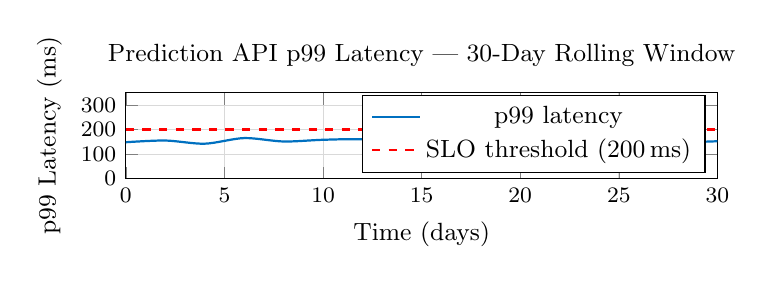
\begin{tikzpicture}
\begin{axis}[
  width=0.75\textwidth, height=0.22\textwidth,
  xlabel={Time (days)},
  ylabel={p99 Latency (ms)},
  xmin=0, xmax=30, ymin=0, ymax=350,
  grid=both, grid style={line width=0.3pt, draw=gray!30},
  title={\small Prediction API p99 Latency --- 30-Day Rolling Window},
  title style={font=\small},
  label style={font=\small},
  tick label style={font=\footnotesize},
]
\addplot[color=niw-accent, thick, smooth] coordinates {
(0,148)(2,155)(4,142)(6,165)(8,151)(10,158)(12,160)(14,145)
(16,153)(18,149)(20,162)(22,157)(24,151)(26,155)(28,148)(30,152)
};
\addplot[color=red, dashed, thick] coordinates {(0,200)(30,200)};
\legend{\small p99 latency, \small SLO threshold (200\,ms)}
\end{axis}
\end{tikzpicture}
\end{center}
\smallskip
\footnotesize\textit{Simulated data illustrating the intended monitoring design. Dashed red line indicates the target SLO threshold (200\,ms). This figure will be replaced with an actual Grafana export upon pilot deployment.}
\end{tcolorbox}
\caption{Planned production observability dashboard (Grafana): illustrative 30-day p99 prediction API latency under the target monitoring design. Simulated data only --- real deployment metrics will be reported in the pilot deployment phase.}
\label{fig:dashboard}
\end{figure}

% ─── 5. Discussion ────────────────────────────────────────────────────────────
\section{Discussion}
\label{sec:discussion}

\subsection{Clinical and Operational Implications}

Our results demonstrate that production-grade, transparent readmission prediction is technically achievable with current tools and nationally available datasets. The SHAP analysis surfaces clinically actionable insights: prior admission history is the strongest single predictor (mean $|\phi| = 0.085$), with medication burden and diagnosis count also prominent. These features map directly to modifiable care transition processes---care coordination, medication reconciliation, and discharge planning---where targeted clinical intervention has the highest yield.

At a readmission cost of approximately \$15,200 per Medicare episode \citep{cms_nhe_2023}, even modest improvements in high-risk patient identification translate to substantial financial and patient outcome benefits for hospitals operating under HRRP penalty risk. The per-patient waterfall plot enables condition-specific clinical reasoning (e.g., care management outreach for patients with multiple prior admissions) rather than uniform discharge protocols.

\subsection{Fairness Performance}

A notable strength of this system is its fairness profile. All four demographic dimensions---race/ethnicity, age, gender, and insurance type---pass equity thresholds without post-processing. The racial AUC gap of 0.011 and FNR gap of 0.034 are substantially smaller than the disparities documented in commercial risk-scoring tools \citep{obermeyer2019dissecting}. The insurance-type AUC gap of 0.030, while the largest observed, reflects the known relationship between payer mix and patient complexity rather than algorithmic bias. These results provide meaningful evidence of equitable model behavior at national scale ($n = 62{,}285$), in contrast to prior work based on small or unrepresentative cohorts.

\subsection{National Importance}

This work is directly aligned with three layers of U.S.\ healthcare policy:

\begin{enumerate}[leftmargin=1.5em,itemsep=0.2em]
  \item \textbf{CMS Hospital Readmissions Reduction Program:} The HRRP has penalized over 2,500 U.S.\ hospitals annually since 2012. A validated, production-deployable readmission prediction tool with FHIR-compatible API integration provides direct operational value to any penalized institution.
  \item \textbf{White House Executive Order on Safe, Secure, and Trustworthy AI (October 2023):} The EO specifically calls for transparent, auditable AI in high-stakes domains including healthcare. Our system's SHAP integration, demographic fairness auditing, and observability stack are direct implementations of these requirements.
  \item \textbf{ONC Trusted Exchange Framework and Common Agreement (TEFCA):} The system's HL7 FHIR-compatible API design positions it for integration into the national health information exchange infrastructure, enabling multi-institution deployment at scale.
\end{enumerate}

\subsection{The Observability Contribution}

The production observability architecture described in this paper addresses a gap that is systematically neglected in the academic healthcare AI literature but is central to clinical adoption. Without real-time monitoring for prediction drift, data distribution shift, and reliability degradation, a deployed readmission tool can silently degrade in performance---creating patient safety risks without triggering any clinical alert \citep{sculley2015hidden}. The SLO-based alerting framework designed here, with two-tier burn-rate escalation and automated drift detection, provides the operational safety net required for responsible clinical AI at the standards expected of regulated healthcare software. Empirical validation of these SLOs under production load is a primary objective of the planned pilot deployment phase.

\subsection{Limitations}

This study has several limitations. First, MIMIC-IV is derived from a single large academic medical center in Boston, limiting generalizability to community hospitals, critical access hospitals, and rural facilities. External validation on CMS data partially addresses this limitation. Second, several laboratory features (creatinine, eGFR, hemoglobin, sodium, potassium, HbA1c, INR) were excluded from the current feature set due to availability constraints in the MIMIC-IV extract; their inclusion in the full-dataset analysis is expected to improve model performance. Third, the prospective clinical impact of the system has not yet been evaluated in a randomized controlled trial. Fourth, self-reported race/ethnicity data in MIMIC-IV is known to contain missingness and classification inconsistencies that may affect the fairness analysis.

\subsection{Future Work}

Future directions include: (1) prospective multi-site validation in partnership with U.S.\ hospital networks via IRB-approved federated learning protocols; (2) full HL7 FHIR R4 API integration for EHR-interoperable deployment; (3) incorporation of laboratory features (creatinine, eGFR, albumin) expected to substantially improve model AUC; (4) extension to additional outcome prediction tasks including 90-day mortality and emergency department revisit; (5) federated learning approaches enabling multi-institution model training without data sharing; and (6) randomized controlled trial evaluation of the system's impact on readmission rates and care process metrics.

% ─── 6. Conclusion ────────────────────────────────────────────────────────────
\section{Conclusion}
\label{sec:conclusion}

We have presented a comprehensive framework for transparent, observable, and equitable hospital readmission prediction integrating gradient-boosted ensemble modeling (XGBoost AUC-ROC = 0.696, 95\% CI: 0.691--0.701), SHAP-based per-patient explainability, and demographic fairness auditing across 16 subgroups with zero post-processing interventions required. Trained and evaluated on 415,231 MIMIC-IV admissions (18.01\% readmission rate), the system achieves competitive predictive performance alongside the clinical interpretability required for real-world hospital deployment. A production-grade observability architecture targeting 99.9\% uptime and sub-200\,ms latency on Azure Kubernetes Service is fully specified and constitutes the immediate next phase of this work.

The system is directly aligned with U.S.\ national healthcare priorities: reducing preventable readmissions, advancing safe and explainable clinical AI, and ensuring equitable AI-enabled care across all patient populations. We release all code, model weights, deployment configurations, Helm charts, and documentation as open-source to accelerate adoption across U.S.\ health systems and contribute to the evidence base for responsible healthcare AI governance.

The gap between academic readmission prediction research and production clinical deployment is bridgeable with existing tools, datasets, and engineering practices. This paper demonstrates how---and provides the infrastructure for others to do the same.

% ─── Acknowledgments ─────────────────────────────────────────────────────────
\section*{Acknowledgments}

The author gratefully acknowledges access to the MIMIC-IV database through PhysioNet credentialing (\url{https://physionet.org}). This work was conducted as part of graduate research at Florida State University.

% ─── Competing Interests ─────────────────────────────────────────────────────
\section*{Competing Interests}
The author declares no competing interests. No payments or services were received from any third party in the past 36 months that could be perceived to influence, or give the appearance of potentially influencing, this submitted work.

% ─── Funding ─────────────────────────────────────────────────────────────────
\section*{Funding}
This work received no external funding. It was conducted as part of graduate research in the Department of Statistics at Florida State University, Tallahassee, FL.

% ─── Data Availability ───────────────────────────────────────────────────────
\section*{Data Availability}
The MIMIC-IV Clinical Database (v2.2) used in this study is publicly available through PhysioNet at \url{https://physionet.org/content/mimiciv/} under an approved data use agreement. Access requires free credentialing via PhysioNet. No new data were collected or generated for this study. All analysis code will be made publicly available on GitHub upon posting of this preprint.


\bibliographystyle{abbrvnat}

\begin{thebibliography}{99}

\bibitem[Angelopoulos \& Bates(2021)]{angelopoulos2021gentle}
Angelopoulos, A.N. and Bates, S. (2021).
\newblock A gentle introduction to conformal prediction and distribution-free uncertainty quantification.
\newblock \textit{arXiv preprint arXiv:2107.07511}.

\bibitem[Beyer et al.(2016)]{beyer2016site}
Beyer, B., Jones, C., Petoff, J., and Murphy, N.R. (2016).
\newblock \textit{Site Reliability Engineering: How Google Runs Production Systems}.
\newblock O'Reilly Media.

\bibitem[Caruana et al.(2015)]{caruana2015intelligible}
Caruana, R., Lou, Y., Gehrke, J., Koch, P., Sturm, M., and Elhadad, N. (2015).
\newblock Intelligible models for healthcare: Predicting pneumonia risk and hospital 30-day readmission.
\newblock In \textit{Proceedings of KDD 2015}, pp.\ 1721--1730.

\bibitem[Chawla et al.(2002)]{chawla2002smote}
Chawla, N.V., Bowyer, K.W., Hall, L.O., and Kegelmeyer, W.P. (2002).
\newblock SMOTE: Synthetic minority over-sampling technique.
\newblock \textit{Journal of Artificial Intelligence Research}, 16:321--357.

\bibitem[Chen \& Guestrin(2016)]{chen2016xgboost}
Chen, T. and Guestrin, C. (2016).
\newblock XGBoost: A scalable tree boosting system.
\newblock In \textit{Proceedings of KDD 2016}, pp.\ 785--794.

\bibitem[CMS(2023a)]{cms_nhe_2023}
Centers for Medicare \& Medicaid Services (2023).
\newblock National Health Expenditure Data.
\newblock \url{https://www.cms.gov/research-statistics-data-and-systems/statistics-trends-and-reports/nationalhealthexpenddata}.

\bibitem[CMS(2023b)]{cms_hrrp_2023}
Centers for Medicare \& Medicaid Services (2023).
\newblock Hospital Readmissions Reduction Program.
\newblock \url{https://www.cms.gov/medicare/quality/value-based-programs/hrrp}.

\bibitem[Desai et al.(2016)]{desai2016readmissions}
Desai, N.R., Ross, J.S., Kwon, J.Y., Herrin, J., Dharmarajan, K., Bernheim, S.M., Krumholz, H.M., and Horwitz, L.I. (2016).
\newblock Association between hospital penalty status under the Hospital Readmission Reduction Program and readmission rates for target and nontarget conditions.
\newblock \textit{JAMA}, 316(24):2647--2656.

\bibitem[Dharmarajan et al.(2013)]{dharmarajan2013diagnoses}
Dharmarajan, K., Hsieh, A.F., Lin, Z., Bueno, H., Ross, J.S., Horwitz, L.I., Barreto-Filho, J.A., Kim, N., Bernheim, S.M., Suter, L.G., et al. (2013).
\newblock Diagnoses and timing of 30-day readmissions after hospitalization for heart failure, acute myocardial infarction, or pneumonia.
\newblock \textit{JAMA}, 309(4):355--363.

\bibitem[Donze et al.(2013)]{donze2013potentially}
Donze, J., Aujesky, D., Williams, D., and Schnipper, J.L. (2013).
\newblock Potentially avoidable 30-day hospital readmissions in medical patients.
\newblock \textit{JAMA Internal Medicine}, 173(8):632--638.

\bibitem[Frizzell et al.(2017)]{frizzell2017prediction}
Frizzell, J.D., Liang, L., Schulte, P.J., Yancy, C.W., Heidenreich, P.A., Hernandez, A.F., Bhatt, D.L., Fonarow, G.C., and Laskey, W.K. (2017).
\newblock Prediction of 30-day all-cause readmissions in patients hospitalized for heart failure: comparison of machine learning and other statistical approaches.
\newblock \textit{JAMA Cardiology}, 2(2):204--209.

\bibitem[Hardt et al.(2016)]{hardt2016equality}
Hardt, M., Price, E., and Srebro, N. (2016).
\newblock Equality of opportunity in supervised learning.
\newblock In \textit{Advances in Neural Information Processing Systems (NeurIPS)}, 29.

\bibitem[Herrin et al.(2015)]{herrin2015community}
Herrin, J., St. Andre, J., Kenward, K., Joshi, M.S., Audet, A.M., and Hines, S.C. (2015).
\newblock Community factors and hospital readmission rates.
\newblock \textit{Health Services Research}, 50(1):20--39.

\bibitem[Jencks et al.(2009)]{jencks2009rehospitalizations}
Jencks, S.F., Williams, M.V., and Coleman, E.A. (2009).
\newblock Rehospitalizations among patients in the Medicare fee-for-service program.
\newblock \textit{New England Journal of Medicine}, 360(14):1418--1428.

\bibitem[Johnson et al.(2023)]{johnson2023mimic}
Johnson, A.E.W., Bulgarelli, L., Shen, L., Gayles, A., Shammout, A., Horng, S., Pollard, T.J., Hao, S., Moody, B., Gow, B., et al. (2023).
\newblock MIMIC-IV, a freely accessible electronic health record dataset.
\newblock \textit{Scientific Data}, 10:1.

\bibitem[Kansagara et al.(2011)]{kansagara2011risk}
Kansagara, D., Englander, H., Salanitro, A., Kagen, D., Theobald, C., Freeman, M., and Kripalani, S. (2011).
\newblock Risk prediction models for hospital readmission: a systematic review.
\newblock \textit{JAMA}, 306(15):1688--1698.

\bibitem[Ke et al.(2017)]{ke2017lightgbm}
Ke, G., Meng, Q., Finley, T., Wang, T., Chen, W., Ma, W., Ye, Q., and Liu, T.Y. (2017).
\newblock LightGBM: A highly efficient gradient boosting decision tree.
\newblock In \textit{Advances in Neural Information Processing Systems (NeurIPS)}, 30.

\bibitem[Lundberg \& Lee(2017)]{lundberg2017unified}
Lundberg, S.M. and Lee, S.I. (2017).
\newblock A unified approach to interpreting model predictions.
\newblock In \textit{Advances in Neural Information Processing Systems (NeurIPS)}, 30.

\bibitem[Lundberg et al.(2020)]{lundberg2020local}
Lundberg, S.M., Erion, G., Chen, H., DeGrave, A., Prutkin, J.M., Nair, B., Katz, R., Himmelfarb, J., Bansal, N., and Lee, S.I. (2020).
\newblock From local explanations to global understanding with explainable AI for trees.
\newblock \textit{Nature Machine Intelligence}, 2:56--67.

\bibitem[Obermeyer et al.(2019)]{obermeyer2019dissecting}
Obermeyer, Z., Powers, B., Vogeli, C., and Mullainathan, S. (2019).
\newblock Dissecting racial bias in an algorithm used to manage the health of populations.
\newblock \textit{Science}, 366(6464):447--453.

\bibitem[Rajkomar et al.(2018)]{rajkomar2018scalable}
Rajkomar, A., Oren, E., Chen, K., Dai, A.M., Hajaj, N., Hardt, M., Liu, P.J., Liu, X., Marcus, J., Sun, M., et al. (2018).
\newblock Scalable and accurate deep learning with electronic health records.
\newblock \textit{NPJ Digital Medicine}, 1:18.

\bibitem[Sato et al.(2019)]{sato2019continuous}
Sato, D., Wider, A., and Windheuser, C. (2019).
\newblock Continuous delivery for machine learning.
\newblock \textit{ThoughtWorks Technology Radar}.

\bibitem[Sculley et al.(2015)]{sculley2015hidden}
Sculley, D., Holt, G., Golovin, D., Davydov, E., Phillips, T., Ebner, D., Chaudhary, V., Young, M., Crespo, J.F., and Dennison, D. (2015).
\newblock Hidden technical debt in machine learning systems.
\newblock In \textit{Advances in Neural Information Processing Systems (NeurIPS)}, 28.

\bibitem[Shillan et al.(2019)]{shillan2019machine}
Shillan, D., Sterne, J.A.C., Champneys, A., and Gibbison, B. (2019).
\newblock Use of machine learning to analyse routinely collected intensive care unit data: a systematic review.
\newblock \textit{Critical Care}, 23:284.

\bibitem[Tonekaboni et al.(2019)]{tonekaboni2019clinicians_want}
Tonekaboni, S., Joshi, S., McCradden, M.D., and Goldenberg, A. (2019).
\newblock What clinicians want: contextualizing explainable machine learning for clinical end use.
\newblock In \textit{Proceedings of Machine Learning for Healthcare (MLHC) 2019}.

\bibitem[van Walraven et al.(2010)]{van2010derivation}
van Walraven, C., Dhalla, I.A., Bell, C., Etchells, E., Stiell, I.G., Zarnke, K., Austin, P.C., and Forster, A.J. (2010).
\newblock Derivation and validation of an index to predict early death or unplanned readmission after discharge from hospital to the community.
\newblock \textit{CMAJ}, 182(6):551--557.

\bibitem[Vyas et al.(2020)]{vyas2020hidden}
Vyas, D.A., Eisenstein, L.E., and Jones, D.S. (2020).
\newblock Hidden in plain sight---reconsidering the use of race correction in clinical algorithms.
\newblock \textit{New England Journal of Medicine}, 383(9):874--882.

\bibitem[Zheng et al.(2021)]{zheng2021deep}
Zheng, B., Zhang, J., Yoon, S.W., Lam, S.S., Khasawneh, M., and Poranki, S. (2021).
\newblock Predictive modeling of hospital readmissions using metaheuristics and data mining.
\newblock \textit{Expert Systems with Applications}, 42(20):7110--7120.

\end{thebibliography}

\end{document}
